
% JuliaCon proceedings template
\documentclass{juliacon}
\setcounter{page}{1}


% Mathematics is necessary
\usepackage{amsmath}
\allowdisplaybreaks

% Physics rules
\usepackage{siunitx}
% \sisetup{output-exponent-marker=\text{e}}
% \sisetup{tight-spacing=true}

% Use multiple images in a single environment
\usepackage{subcaption}

% Plotting in tikz images
\usepackage{pgfplots}
% Silence warnings
\pgfplotsset{compat=1.16}
% Allow external generation of images to speed up compilation
% \usetikzlibrary{external}
% \tikzexternalize[prefix=../figures/tikz/]

% Macros
\usepackage{xspace}
\newcommand{\ca}[0]{{ca.\@}\xspace}
\newcommand{\cf}[0]{{cf.\@}\xspace}
\newcommand{\eg}[0]{{e.g.\@}\xspace}
\newcommand{\ie}[0]{{i.e.\@}\xspace}
\newcommand{\etc}[0]{{etc.\@}\xspace}
\newcommand{\trixi}{Trixi.jl\xspace}


\begin{document}

\input{header}

\maketitle

\begin{abstract}
% Abstract: at most 600 characters, written in plain English with no symbol
% nor formula + references etc.
We present Trixi.jl, a Julia library for adaptive high-order numerical simulations
of hyperbolic partial differential equations (PDEs). Utilizing Julia's strengths,
Trixi.jl is extendable, easy to use, and fast. We describe the main design choices
that allow satisfying these goals and compare Trixi.jl with an established open
source Fortran code for hyperbolic PDEs using the same numerical methods.
We conclude with an assessment of Julia for simulation-focused scientific
computing, an area that is still dominated by traditional high-performance
computing languages such as C, C++, and Fortran.
\end{abstract}


\section*{TODO}

\begin{itemize}
  \item Basic design of \trixi and its capabilities
  \item PID comparison of Fluxo and \trixi
  \item Discussion: Julia for numerical simulation science
  \item Prepare repro repo including scripts for \trixi and Fluxo
  \item Cite \cite{bezanson2017julia,schlottkelakemper2021purely,rackauckas2017differentialequations,revels2016forward,ranocha2021sbp}
  \item The title of our talk at JuliaCon is
  ``Adaptive and extendable numerical simulations with Trixi.jl''.
  Shall we use something like
  ``Adaptive high-order numerical simulations of hyperbolic PDEs with Trixi.jl:
  A case study of Julia for scientific computing'' for this paper?
  \item Restructure non-conservative stuff and add MHD benchmarks?
  \item Shall we re-create the schematic overview in tikz?
\end{itemize}


\section{Introduction}

\trixi\footnote{https://github.com/trixi-framework/Trixi.jl} provides adaptive
high-order numerical simulations of hyperbolic partial differential equations (PDEs).
in Julia \cite{bezanson2017julia}.

TODO %TODO


\section{Design of \trixi and overview of its features}

\trixi is designed as a library of high-order methods for hyperbolic PDEs of
the form
\begin{equation}
\label{eq:hcl}
  \partial_t u(t, x) + \sum_{j=1}^d \partial_{x_j} f^j(u) = s(t, x, u),
  \quad t \in (0, T), x \in \Omega,
\end{equation}
in $d \in \{1, 2, 3\}$ space dimensions. Here, the independent variables are
time $t$ and space coordinates $x \in \Omega \subset \mathbb{R}^d$. The conserved
quantities are denoted as $u$, \eg, mass, momentum, and energy for the compressible
Euler equations of an ideal gas.
The physical model is specified by the fluxes $f^j$ and the source term $s$.
In addition, suitable initial and boundary conditions (ICs, BCs) are required.
\trixi also handles non-conservative source terms containing derivatives of the
conserved quantities as in the shallow water equations or magnetohydrodynamics
with divergence cleaning.

\subsection{High-level overview of the structure}

\trixi is based on the method of lines. Thus, a discretization of \eqref{eq:hcl}
is obtained in two steps. First, a spatial semidiscretization is created. Next,
the resulting ordinary differential equation (ODE) is solved using a time
integration method. Currently, \trixi focuses on the spatial semidiscretization
and uses mostly Runge-Kutta methods implemented in OrdinaryDiffEq.jl, a part
of DifferentialEquations.jl \cite{rackauckas2017differentialequations}.

\begin{figure*}
  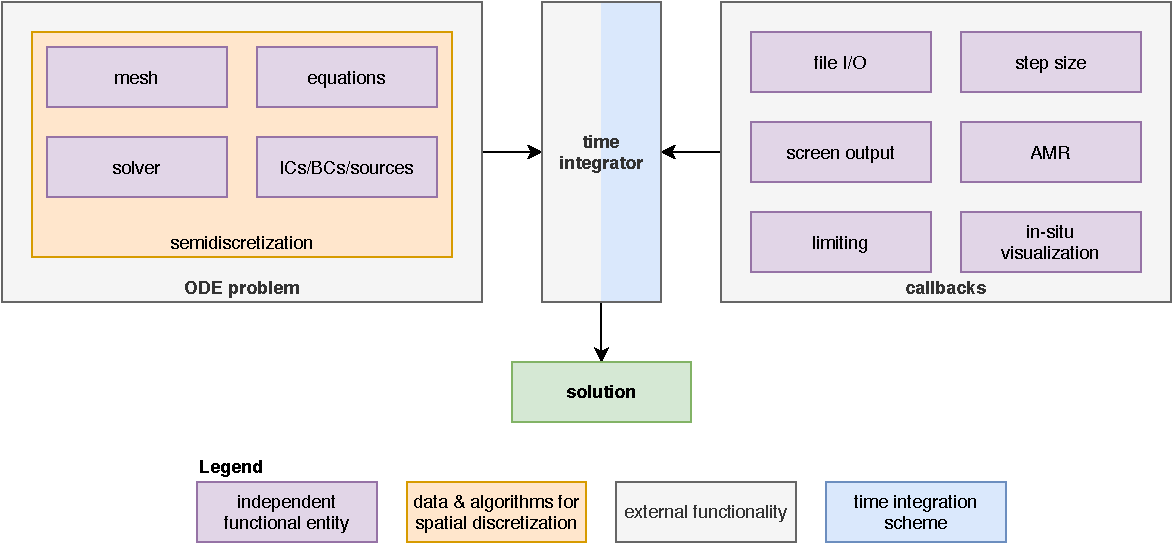
\includegraphics[width=\linewidth]{../figures/trixi_global_overview}
  \caption{Schematic overview of the basic components of \trixi and how they
           interact with each other.}
  \label{fig:trixi_global_overview}
\end{figure*}

Figure~\ref{fig:trixi_global_overview} presents an overview of the basic
components of \trixi. The most important structure is the semidiscretization,
which bundles all information about the spatial part. The mathematical-physical
model is determined by the \lstinline{equations}, the \lstinline{initial_condition},
\lstinline{boundary_conditions}, and possible \lstinline{source_terms}. The
\lstinline{solver} describes purely numerical parameters determining the specific
discretization method such as discontinuous Galerkin or finite difference
methods, kinetic energy preserving or shock capturing approaches. Finally, the
\lstinline{mesh} has a necessarily hybrid role including information about the
spatial domain and its discretization.

Adding information about the time span $[0, T]$, a semidiscretization of \trixi
can be converted into an ODE problem, which can be solved by methods from
OrdinaryDiffEq.jl. The flexible callback infrastructure of this ODE library
allows us to provide extended functionality for \trixi without modifying any
main loop. In particular, diverse tasks such as input/output operations, adaptive
mesh refinement (AMR), and positivity preserving limiting are implemented using
callbacks.

\subsection{Main features of \trixi}

TODO %TODO



\section{Performance comparison with FLUXO}

FLUXO\footnote{\url{https://gitlab.com/project-fluxo/fluxo}} is an open source
MPI Fortran code implementing discontinuous Galerkin methods on unstructured hex
meshes in three space dimensions for advection diffusion equations. It also
implements the same kind of modern DG methods based on flux differencing
to achieve entropy conservation/dissipation or kinetic energy preservation.
Thus, both \trixi and FLUXO share a common set of features, enabling a reasonable
comparison of their performance.

Here, we compare the serial performance of \trixi and FLUXO when solving a
hyperbolic PDE in three space dimensions on curvilinear hex meshes.

TODO: Andrew, please describe the setups that you used. %TODO

The results of this comparison are visualized in Figure~\ref{fig:PID-Euler}.
Clearly, \trixi is more than 2x faster than the Fortran code FLUXO
while both implement the same numerical methods. This demonstrates the
suitability of Julia for this kind of simulation-focused scientific computing.

\begin{figure}
\centering
  \begin{subfigure}{\linewidth}
    \begin{tikzpicture}[
      font=\footnotesize
      ]
      \begin{axis}[
          xlabel={Polynomial degree},
          % ylabel={Time per RHS call and DOF (seconds)},
          ylabel={Time/RHS/DOF {[sec]}},
          width=\textwidth,
          height=0.66\textwidth,
          legend columns=-1,
          % legend to name=place_legend_here,
          legend pos=north west,
          ymin=0.0,
          ymax=2.2e-6,
          grid=major,
        ]
        \addplot[blue, mark=*, solid] % FLUXO, weak form
          table [x index=0, y index=3]{../data/pids_euler_weak.dat};
          \addlegendentry{FLUXO}
%         \addplot[orange, mark=square*, solid] % TreeMesh, weak form
%           table [x index=0, y index=1]{../data/pids_euler_weak.dat};
%           \addlegendentry{\texttt{TreeMesh} (\trixi)}
        \addplot[red, mark=diamond*, solid] % StructuredMesh, weak form
          table [x index=0, y index=2]{../data/pids_euler_weak.dat};
          % \addlegendentry{\texttt{StructuredMesh} (\trixi)}
          \addlegendentry{\trixi}
        \node at (axis cs:13,3.5e-7) {Weak form};

        \addplot[blue, mark=*, dashed] % FLUXO, flux differencing
          table [x index=0, y index=3]{../data/pids_euler_ranocha.dat};
%         \addplot[orange, mark=square*, dashed] % TreeMesh, flux differencing
%           table [x index=0, y index=1]{../data/pids_euler_ranocha.dat};
        \addplot[red, mark=diamond*, dashed] % StructuredMesh, flux differencing
          table [x index=0, y index=2]{../data/pids_euler_ranocha.dat};
        \node [rotate=23] at (axis cs:9,8.2e-7) {Flux differencing};
        \draw (axis cs:9,9.2e-7) -- (axis cs:7.5,10.2e-7);
        \draw (axis cs:9,7.2e-7) -- (axis cs:8.5,5.2e-7);
      \end{axis}
    \end{tikzpicture}%
    \caption{Absolute run times.}
  \end{subfigure}%
  \\
  \begin{subfigure}{\linewidth}
    \begin{tikzpicture}[
      font=\footnotesize
      ]
      \begin{axis}[
          xlabel={Polynomial degree},
          % ylabel={Time per RHS call and DOF (relative)},
          ylabel={Time relative to FLUXO {[-]}},
          width=\textwidth,
          height=0.66\textwidth,
          legend columns=-1,
          legend pos=south west,
          ymin=0.0,
          ymax=1.1,
          ytick={0, 0.2, 0.4, 0.5, 0.6, 0.8, 1},
          grid=major,
        ]
        \addplot[blue, mark=*, solid, forget plot] % FLUXO, weak form
          table [x index=0, y index=3]{../data/pids_euler_weak_relative.dat};
%         \addplot[orange, mark=square*, solid, forget plot] % TreeMesh, weak form
%           table [x index=0, y index=1]{../data/pids_euler_weak_relative.dat};
        \addplot[red, mark=diamond*, solid] % StructuredMesh, weak form
          table [x index=0, y index=2]{../data/pids_euler_weak_relative.dat};
          \addlegendentry{Weak form}

        \addplot[blue, mark=*, dashed, forget plot] % FLUXO, flux differencing
          table [x index=0, y index=3]{../data/pids_euler_ranocha_relative.dat};
%         \addplot[orange, mark=square*, dashed, forget plot] % TreeMesh, flux differencing
%           table [x index=0, y index=1]{../data/pids_euler_ranocha_relative.dat};
        \addplot[red, mark=diamond*, dashed] % StructuredMesh, flux differencing
          table [x index=0, y index=2]{../data/pids_euler_ranocha_relative.dat};
          \addlegendentry{Flux differencing}
      \end{axis}
    \end{tikzpicture}
    \caption{Run time relative to FLUXO.}
  \end{subfigure}%
  \caption{Run time per right-hand side evaluation and degree of freedom for
           different DG discretizations of the 3D compressible Euler equations.}
  \label{fig:PID-Euler}
\end{figure}

Note that we do not want to state that Julia is generically faster than Fortran,
C, or C++. In contrast, we would like to emphasize that Julia can be at least
as fast as code written in these traditional scientific computing languages.
We believe that it will be possible to get the same efficiency by rewriting
FLUXO appropriately. However, the code introspection and profiling tools available
in Julia make it easier for us to optimize Julia code compared to other languages
we are familiar with (having a diverse team with a strong background in C, C++,
and Fortran).

Finally, the different mesh types available in \trixi allow further optimizations.
For example, if the computational domain is essentially a cube (or square, line)
without need for curvilinear coordinates, the Cartesian \lstinline{TreeMesh} can
be used. Depending on the relative computational effort of the discretization
(such as the polynomial degree and the choice of the volume terms), the
Cartesian \lstinline{TreeMesh} can be \ca \SI{10}{\percent}--\SI{25}{\percent}
more efficient than the curvilinear meshes in \trixi.

TODO: Plot of this comparison with the \lstinline{TreeMesh}?



\section{Assessment of Julia for simulation-focused scientific computing}

TODO %TODO
\begin{itemize}
  \item Packages can really be used together at low (or no) cost
  \item Reproducibility
  \item Good software development practices (CI, tests, version management)
  \item Relatively easy to integrate existing C libraries (p4est, HDF5)
  \item more nice features
  \item Can be extended: Multi-physics with 350 lines of code
  \item Compilation time can be annoying but also allows cool features and performance \cite{schlottkelakemper2021purely}
  \item MPI: To be evaluated but the basic tools are already there \cite{byrne2021mpi}
\end{itemize}



\section{Summary and conclusions}

TODO %TODO



\section*{Acknowledgments}

Funded by the Deutsche Forschungsgemeinschaft (DFG, German Research Foundation)
under Germany's Excellence Strategy EXC 2044-390685587, Mathematics Münster:
Dynamics-Geometry-Structure.

TODO: Add your funding sources (if any) %TODO


% References
% **************GENERATED FILE, DO NOT EDIT**************

\bibliographystyle{juliacon}
\bibliography{ref.bib}




\clearpage
\section*{Some guidelines}
\label{sec:some_guide}

Full paper: 5--10 pages.
\begin{quote}
  Compared to an extended abstract, a full paper presents more of the background
  and context motivating the work. It compares the work to other approaches taken
  in the field and gives some additional insights on the conference contribution.
  Use cases back up the work by showing how it can be used.
\end{quote}


The following notes may help you achieve the best effects with the
\verb juliacon  class file.

\subsection{Writing Julia code}

A special environment is already defined for Julia code,
built on top of \textit{listings} and \textit{jlcode}.

\begin{verbatim}
\begin{lstlisting}[language = Julia]
using Plots

x = -3.0:0.01:3.0
y = rand(length(x))
plot(x, y)
\end{lstlisting}
\end{verbatim}
\begin{lstlisting}[language = Julia]
using Plots

x = -3.0:0.01:3.0
y = rand(length(x))
plot(x, y)
\end{lstlisting}

\subsection{Double Column Figure and Tables}
\label{subsub:double_fig_tab}
For generating the output of figures and tables in double column
we can use the following coding:

\begin{enumerate}
\item For Figures:
\begin{verbatim}
\begin{figure*}...\end{figure*}
\end{verbatim}
\item For landscape figures:
\begin{verbatim}
\begin{sidewaysfigure*}...\end{sidewaysfigure*}
\end{verbatim}
\item For Tables:
\begin{verbatim}
\begin{table*}...\end{table*}
\end{verbatim}
\item For landscape tables:
\begin{verbatim}
\begin{sidewaystable*}...\end{sidewaystable*}
\end{verbatim}
\end{enumerate}

\subsection{Enunciations}
\label{subsub:enunciation}

The \verb juliacon   class file generates the enunciations with the help of
the following commands:
\begin{verbatim}
\begin{theorem}...\end{theorem}
\begin{strategy}...\end{strategy}
\begin{property}...\end{property}
\begin{proposition}...\end{proposition}
\begin{lemma}...\end{lemma}
\begin{example}...\end{example}
\begin{proof}...\end{proof}
\begin{definition}...\end{definition}
\begin{algorithm}...\end{algorithm}
\begin{remark}...\end{remark}
\end{verbatim}
The above-mentioned coding can also include optional arguments
such as
\begin{verbatim}
\begin{theorem}[...]. Example for theorem:
\begin{theorem}[Generalized Poincare Conjecture]
Four score and seven ... created equal.
\end{theorem}
\end{verbatim}

\begin{theorem}[Generalized Poincare Conjecture]
Four score and seven years ago our fathers brought forth,
upon this continent, a new nation, conceived in Liberty,
 and dedicated to the proposition that all men are
created equal.
\end{theorem}


\subsection{Balancing column at last page}
\label{subsub:Balance}
For balancing the both column length at last page use:
\begin{verbatim}
\vadjust{\vfill\pagebreak}
\end{verbatim}

% \vadjust{\vfill\pagebreak}

at appropriate place in your \TeX{} file or in bibliography file.

\end{document}

% Inspired by the International Journal of Computer Applications template
